% !TEX root = ../../report.tex
\section{The Cold-start Problem}

%Can the different approaches be classified? E.g. 3 main categories of approaches
    %Initial categorization
        %Interview process
        %Hybrid approaches
        %Key figures / Seed users
        %Filterbots
        %Trust-aware / Trust propagation

In the literature, the term cold is used about an object in a system, or a
whole system, which is new \cite{Schein2002, Park2006}. Cold-start scenarios in recommender systems are
situations in which little/no prior events, like ratings or clicks, are known
for certain users or items. The cold-start problem can be divided into three sub problems:

\begin{itemize}
  \item \emph{Cold-start system}: A situation where we only have new users and
  little or no ratings for the items.

  \item \emph{Cold-start item}: The problem of recommending items that are new
  to the system, which have not received any ratings.

  \item \emph{Cold-start user}: The problem of giving accurate recommendations
  to a user who is new to a recommender system.
\end{itemize}


For example in a scenario where the average item in an item collection have 5
000 ratings, a new item with only 5 ratings would be considered a
\emph{cold-item}. Likewise, in a recommender system where the average user has
rated 25 items, a user who only has rated 2 items, would be considered a
\emph{cold-user}.

The cold-start system problem is mainly a collaborative filtering problem, and
can be seen as a combination of the cold-start user and cold-start item problem
where the majority of the users are new to the system and have expressed few
preferences, resulting in a very sparse user-item matrix, rendering traditional
collaborative-filtering methods futile. Most traditional algorithms only work
effectively in environments where the datasets has high information density. In
fact, in extreme cases, when data is very scarce, simple non-personalized
recommendations based on global averages can outperform collaborative-filtering
algorithms \cite{Park2006}. The reason why the cold-start system problem is not
so evident in content-based systems is due to \emph{User Independence}, meaning
that the system only exploits ratings provided by the active user to build her
profile. Instead, collaborative filtering methods need ratings from other users
to find the "peers" of the active users.

In content-based systems, new items can easily be recommended using the content
information of the item, making it a popular solution to the \emph{cold-start
item} problem. This problem is more severe in collaborative-filtering systems
where items are only recommendable if they have been rated by substantial
amount of users. New items will therefore not be recommendable before multiple
users somehow stumble upon the new item while e.g. browsing the item
collection, unless additional measures are taken to solve this problem. To
\emph{solve} the new-item problem, there are two commonly used (simple)
solutions often used in E-commerce websites:

\begin{itemize}

\item Advertising at the front-page of the website, putting the new items in an
eye catching position. This solution, however, may this result in that some
users, which don't like these new items, might leave the website.
\item Requesting the user to choose one or more of his/hers categories while
registering for the site, and recommend items from the selected categories.
This approach however, requires active user involvement and complicates the
sign up process. Many users might chose not to give up any personal interest
information, thus the user group covered by this solution could end up not
being large enough.
\end{itemize}

The cold-start user problem is present both in content-based and collaborative-filtering systems.
Collaborative Filtering is based on the idea that like-minded users have similar tastes and preferences.
A new user therefore poses a challenge to a CF recommender, since the system has no knowledge about
the preferences of the new user, and can therefore not provide any personalized recommendations. The system must therefore acquire some
information about the new user before it can start making personalized recommendations. In a typical domain, for example in the domain of books, the number of items is very large (in the order of tens of thousands) while the number of items rated by every single user is in general small (in the order of dozens or less). This means that it is very unlikely two random users have rated any items in common and hence they are not comparable. The system will therefore most likely struggle to find users with tastes that are \emph{truly} similar to the target user. Similarly, in content-based systems, the lack of ratings given by the target user, means that the target user will have a limited
content-profile, since the users content profile is constructed using content-information from his/hers rated items. In both cases, recommendation quality is most likely bound to suffer.\newline

This section will present a few different solutions to the cold-start problem, focusing mainly on \emph{complete} solutions to the cold-start problem.

\subsection{Trust Aware Recommender Systems}

One promising direction to solve the cold-start problem is the incorporation of
a trust network. A trust network can significantly help alleviate the
cold-start user problem, primarily since the trust statements between users can
be propagated and aggregated, and consequently connect more people and
products. By making clever connections in the trust network, newcomers can
immediately gain access to a wide range of connections.


%Due to the popularity of social networks such as Facebook, more and more
%researchers turn to incorporate the social relationships (e.g. trust) of users
%to help complement users’ preference in addition to item ratings, in order to overcome the limitations of existing recommender systems

For example, when looking for movie recommendations we often turn to our friends which we share a similar taste in movies with. Trust can be defined as: "believe in the reliability, truth, or ability of", and in the context of recommender systems a trusted user would be a user you trust to provide you with good recommendations. E.g. in the case of the Epinions dataset \cite{Epinions}, users can explicitly state whether they trust or distrust a user [1, -1], i.e. reviewers whose reviews and ratings they have consistently found to be valuable or reviewers which they find consistently offensive, inaccurate or not valuable. In decentralized environments where everyone is free to create content and there
is no centralized quality control entity, evaluating the quality of the content becomes an important issue. This phenomenon can be observed in online
marketplaces such as E-bay where users can create "fake" auctions and in peer-to-peer networks where peers can enter corrupted items. In these environments, it is often a good strategy to delegate the quality assessment task to users themselves. E.g. \emph{Ebay.com} allows users to express their level of satisfaction after every interaction with another user. Trust relationships of users are often employed in order to correlate more potential raters for the active users who require recommendations \cite{Massa2004, Massa2007}. Massa et. al. \cite{Massa2004} also show that some of the weaknesses of recommender systems such as data sparseness and their susceptibility to shilling attacks could be alleviated by incorporating trust.

% The formals
In \cite{Massa2004}, Massa et al. proposes a Trust-Aware recommender system
architecture.  To capture all the trust statements we need a $CxC$ matrix,
where $C$ is the number of users, since each user is allowed to express a trust
value in every other user. This matrix will make up our trust network among the
users. If $u$ trusts $v$, then there is a value $t_{u,v}$ for this trust which
is a real number in $[0,1]$. Zero means no trust and one means full trust. This
additional information can be organized in a trust network and a \emph{trust
metric} can be used to predict the trustworthiness of other users as well (for
example, friends of friends). The idea here is to not search for similar users
as CF does but to search for trust-able users by exploiting trust propagation
over the trust network. The items appreciated by these users are then
recommended to the active user.

% Web of Trust - Figure explanation
Consider the example shown in Figure \ref{figure:weboftrust}. User $A$ has
issued a trust statement in $B$ and $C$; hence $B$ and $C$ are in the web of
trust of $A$. Using these explicit trust statements, it is possible to predict
trust in unknown users by propagating trust, making it possible to infer
something about how much user $A$ could trust $D$.

\begin{figure}[H]
    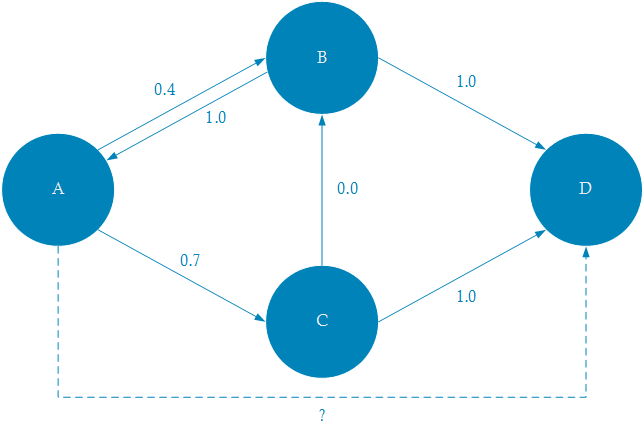
\includegraphics[width=2in]{image/webofTrust.png}
    \centering
    \caption[Trust Network]{Trust Network. Nodes are users and solid edges are trust statements. The dotted edge is one of the undefined and predictable trust statements (Adopted from \cite{Massa2004})}
    \label{figure:weboftrust}
\end{figure}

In addition to the trust network we will also have a rating matrix of size
$CxS$, where $S$ is the number of items. This rating will not differ from a
standard rating matrix, which are used in traditional collaborative filtering
systems. The value $u(c,s)$, is the rating given by user $c$ to item $s$, the
rating scale may differ from system to system.

% Architecture
The systems takes as input the trust network and the ratings matrix and
produces, as output, a matrix of predicted ratings that the users would assign
to the items. Figure \ref{figure:trustarchictecture} shows a conceptual
overview of the trust-aware recommender system architecture.

\begin{figure}[H]
    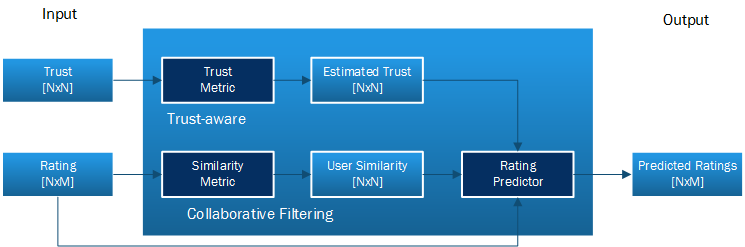
\includegraphics[width=5in]{image/trustawarearchitecture.png}
    \centering
    \caption[Trust-Aware Recommender System Architecture]{Trust-Aware
    Recommender System Architecture (Adopted from \cite{Massa2004})}
    \label{figure:trustarchictecture}
\end{figure}

The \emph{Trust Metric} module takes the trust network as input, and exploits
trust propagation in order to predict, for every user, how much she could trust
other users. Trust metrics can either be local and global. Global trust metrics
produces an estimated trust matrix with all the rows equal, meaning that the
estimated trust in a certain user (column) is the same for every user (row). A
simple local trust metric could e.g. for each user assign to every other user a
predicted trust based on her minimum distance from the source user. More
sophisticated ones could also be employed. If we again consider Figure
\ref{figure:weboftrust}, we could employ a local trust metric where the
predicted trust is based on the minimum distance from the source user. If we
set the maximum propagation distance $d$, a user at distance $n$ from the
source user will have a predicted trust value of:

\begin{equation}
t_{u,v} = (d-n+1)/d
\end{equation}

Giving users not reachable within the maximum propagation distance a trust of
$0$. Using user $A$ as the source user, the users at distance $1$ ($B$ and $C$)
would get a trust value of $(4-1+1)/4 = 1$, while the user at distance 2 (D)
would get a predicted trust value of $(4-2+1)/4 = 0.75$. Meaning that we will
have a linear decay in trust based on the distance from the source user.

Massa et al. \cite{Massa2007} experimented with both local and global trust
metrics. They used the PageRank algorithm as a global trust metric. PageRank
tries to infer the authority of every single user by examining the structure of
the network. The algorithm follows a simple idea: if a link from user $A$ to
user $B$ represent a positive vote casted by $A$ to $B$, then the global rank
of a page depends on the number (and quality) of the incoming links. The trust
values assigned by users to users are used to predict the trustworthiness of
unknown users. Their findings, not surprisingly, indicate that Global Trust
Metrics are not suited for the task of finding good neighbours, especially for
providing personalized recommendations, but is more suited to applications such
as \emph{Ebay.com} to find untrustworthy users. As a local trust metric they
used MoleTrust, which is a depth-first graph walking algorithm with a tuneable
trust horizon which allowed them to experiment with different propagation
distances. They found trusted users to be good predictors. For the cold-start
users they achieved a MAE of 0.674 when looking at friends of friends, compared
to traditional collaborative filtering which scored 1.094. The difference is
very high, and particularly relevant as it is important for recommender systems
to generate personalized recommendations as soon as possible for new users, so
that these users appreciate the system and keep using it.

The \emph{Similarity Metric} module computes the user similarities, this is one
of the standard steps of any traditional collaborative filtering technique,
user similarities can be found e.g. by using the Pearson Correlation
Coefficient. The intuition is that, if a user rates in a similar way to another
user, then her ratings are using for predicting the ratings for that users.

The \emph{Rating Predictor} can use the neighbours from the user similarity
matrix, the estimated trust matrix or a combination of both in order to
calculate the predicted ratings.

% Using a Trust Network to Improve Top-N Recommendation


Jamali et al. \cite{Jamali2009} propose two different methods for getting
around the cold-start user problem using a trust network. Their first approach
called \emph{Random Walk} only utilize the trust network to provide
recommendations. Starting from the active user $u$, we perform a random walk on
the trust network. Each random walk stops at a certain user. Then the items
rated highly by that user will be considered as recommended items, ordered
according to the ratings expressed by that user. Several random walks are
performed to gather more information and compute a more confident result. The
estimated rating of each item is the average of ratings for that item over all
raters considered. At the end, we output items with the highest estimated
rating as top-N recommended items. Their second approach called \emph{Combined
Approach} uses both user-user similarities and the trust network to provide
recommendations. In this approach we compute the top $K$ trusted users in the
network and rank the items rated by these trusted users to compute top-N
recommended items. The top $K$ trusted users can either be found by
\emph{Breadth First Search} or \emph{Random Walk in the social network}. We use
the collaborative filtering approach to compute another set of top-N
recommended items. Finally, we merge these two lists to produce a combined list
of top-N recommended items. Items returned by CF is denoted as $CF_{u}$, while
the items returned by Trust-based approach are denoted $TR_{u}$.

\begin{equation}
 \hat{u}(c,s) =
  \begin{cases}
   \frac{u_{tr_{c,i}}+u_{cf_{c,i}}}{2}     & i \in TR_{u};i \in CF_{u}         \\
   \hat{u_{tr_{c,i}}}                      & i \in TR_{u};i \not \in CF_{u}    \\
   \hat{u_{cf_{c,i}}}                      & i \in CF_{u};i \not \in TR_{u}     \end{cases}
\end{equation}

The top-N items with the highest value of $\hat{u}(c,s)$ will be returned as
the top-N recommended items. The authors also experimented with weighted
averaging in the case where the item appear in both $TR_{u}$ and $CF_{u}$.

The top-N items with the highest value of $\hat{u}(c,s)$ will be returned as
the top-N recommended items. The authors also experimented with weighted
averaging in the case where the item appear in both $TR_{u}$ and $CF_{u}$.
Their approaches showed great improvements in recall for cold-start users,
improving the performance by 50\% over standard CF methods. The main
improvements however, are the coverage of the trust-based approaches, while
still maintaining the same or even slightly better precision than the standard
CF methods.

% Trust-aware Recommender Systems + Trust-Aware Collaborative Filtering for Recommender Systems
% Article Comments:
%   Requires user involvement (explicitly express trust) - is this a acceptable?

%Massa et al. \cite{Massa2004, Massa2007} propose using trust information
%explicitly expressed by the users. Users are allowed to state how much they
%consider every other user trustworthy that, in the context of recommender
%systems, is related to how much they consider the ratings provided by a certain
%user valuable and relevant.

% Alleviating the Sparsity Problem of Collaborative Filtering Using Trust Inferences
% Article Comments:
%   - Pretty good general model for dealing with sparsity
%   - Requires no additional information such as product details, demographic information about userstrus


Papagelis et al. \cite{Papagelis2005} proposed to alleviate sparsity using
trust inferred from user-user similarity. This approach does therefore not
require users to explicitly express their trust in other users, unlike the
approaches described above, the trust information is inferred from the
underlying social network of the rating matrix. Their approach is based on the
assumption that the more similar two users are, the greater their established
trust would be considered.

\begin{figure}[H]
    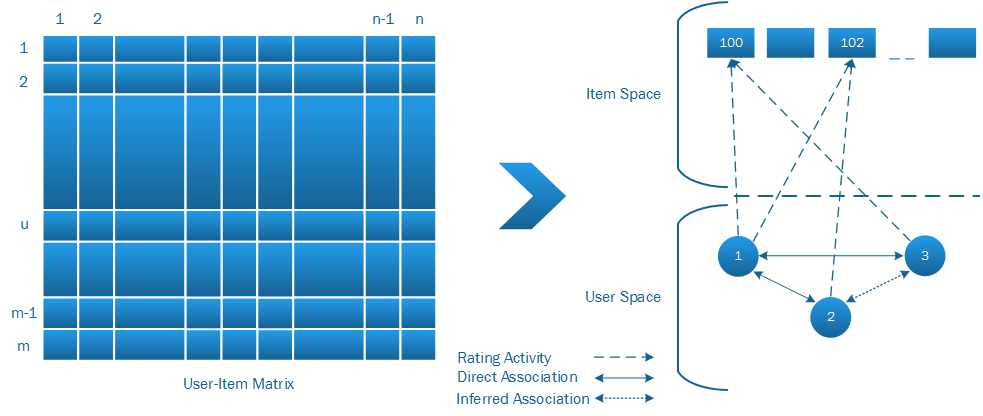
\includegraphics[width=5in]{image/trustnetwork.png}
    \centering
    \caption[Underlying Social Networks in Recommender Systems]{Underlying Social Networks in Recommender Systems}
    \label{figure:cfsocialnetwork}
\end{figure}

Due to the number of ratings that exist in recommendation systems, underlying
social networks are very sparse. There are cases in which insufficient or loss
of information is detrimental for the recommendation algorithms. Consider
Figure \ref{figure:cfsocialnetwork}, classic CF will associate only the users
which have co-rated an item (User $1$ and $2$ and user $1$ and $3$). To deal
with the problem of a sparse social network, it is possible to infer trust
between a source user $S$ and a target user $T$ through an intermediate user
$N$ (User $2$ and $3$ are connected through the intermediary user $1$), as
shown by the \emph{Inferred Association} arrow. According to this process,
trust is propagated in the network and associations between users are built,
even if they have no co-rated item. Trust paths can be of variable length,
depending on the number of associations that one needs to traverse in order to
reach the target user.

% Trust-paths
For example, if the trust $t_{(1,2)} = 0.7$ based on 5 co-rated items
and $t_{(1,3)} = 0.35$ based on 2 co-rated items, then the trust
between user $2$ and $3$ through $1$ is, $\frac{0.7*5}{5+2} + \frac{0.35*2}{7} = 0.6$.

In order to express the subjective notion of trust, the authors set up a
confidence model that is assigned to each direct association of the network
that expresses the reliability of the association. Confidence is related to the
number of co-rated items between two users. The confidence scores are all
expressed in relation to the most confident association for each user.

\begin{equation}
c_{(s,t)} = \frac{n(I_{s} \cap I_{t})}{n(I_{s} \cap I_{u_{MAX_CONF}})}
\end{equation}

Using the above example, assuming that the maximum number of co-rated items
user $1$ has with any user is 7, $c_{(1,2)} = \frac{5}{7}$.

% Results/Findings
The authors achieved improved accuracy for all sparsity levels. With a sparsity
level of $99.9\%$ the 2-HOP CF (friend of friends) increased the MAE
performance by $17\%$ over standard CF methods.

%TODO - READ: A Matrix Factorization Technique with Trust Propagation for Recommendation in Social Networks
%Jamali et al. propose a technique for incorporating trust using matrix factorization, called SocialMF.
%Leverage regularization model to fusing the one mode data by minimizing the gap between the taste of a user and the taste of her trusted friends
%In their model, the users which have not expressed any ratings feature vectors will be learned to be close to their trusted neighbors.

Victor et al. \cite{Victor2008} points out that cold-start users not only have
expressed few ratings, but also typically have expressed trust in few users. In
order for trust-aware recommenders to help cold-start users they need to have
expressed trust in atleast one user. But choosing who to connect to is often a
difficult task. To help cold-start users find trusted users, Victor et al.
propose using key figures or mavens (users who write many reviews), frequent
raters (users who evaluate many items) and connectors (users with
many trust connections). By connecting to these key figures, cold-start users
shown a significant increase in coverage while still maintaining good accuracy.
They also show that connecting to key figures are more beneficial to a
cold-start user than connecting to a random user.

\subsection{Filterbots}

% Na¨ıve Filterbots for Robust Cold-Start Recommendations

Park et al. \cite{Park2006} propose using filterbots to improve the cold-start
performance of collaborative filtering methods. Their filterbots are a varition
of RipperBots, described in detail in \cite{Good1999}. A filterbot is an
automated agent that rates all or most items using information filtering (IF)
techniques. The filterbots injects psuedo users or bots into the system. These
bots rate items algorithmically according to item features and user profiles.
For their movie recommendation systems the authors used 7 global bots which
e.g. rated movies based on average item rating, a critic bot that generates ratings
based on the average critic (pre-selected users) ratings, an award bot that
generates rating based on the awards a movie has won, and so on. These ratings
generated by these bots are injected into the user-item matrix along with
actual user-item ratings. Standard CF algorithms are then applied to generate
recommendations.

Their approach clearly demonstrated better robustness to all three cold-start situations than standard item-based
and user-based collaborative filtering. The improvements were most evident on
the datasets with a high degree of sparsity.

\subsection{Wisdom of the better few / Seed users}

% Wisdom of the Better Few: Cold Start Recommendation via Representative based Rating Elicitation

Liu et al. \cite{Liu2011} propose an approach in which they elect a few
representative users and items. The representative set should represent a set
of active users or items who well represent the entire population but with
little taste overlap. In their approach they wish to find a rank-k
factorization of the form $Y \approx XR$ or $Y \approx CX$ where $X$ is a
loading matrix consisting of free parameters and $R$ and $C$ which is the
component matrix consisting of actual rows or columns from $Y$. The
representative users and items are found using dimensionality reduction
techniques by reducing the column space of the rating matrix from $m$ to $k$.
And then applying basis selection based on the maximum-volume principle to
select the $k$ most representative users or items. In order to be able to
recommend new items to the users it must first be rated by the $k$
representative users, likewise for new users to be rated they need to rate the
$k$ most representative items. Their method therefore easily allows new users
and items to be \emph{folded in}.

\subsection{Intelligent Selection / Interview Process}\mbox{}\\

\begin{chapquote}[30pt]{Vanessa Redgrave}
  "Ask the right questions if you're going to find the right answers"
\end{chapquote}

% Getting to Know You: Learning New User Preferences in Recommender Systems

As pointed out by Rashid et al. \cite{Rashid2002}, the most direct way of
acquiring information for use in personalized recommendations from a new users
is to present item for the user to rate. However, they argue that the system
must be careful to present useful items to garner information. A food
recommender should probably not ask whether a new user likes vanilla ice cream
since most people like vanilla ice cream. Therefore, knowing that a new user
likes vanilla ice cream tells you very little about the user. The choice of
what questions to ask a new user, then, is critical. The authors performed a
study of different item selection strategies that collaborative filtering
recommender systems can use to learn about new users. They presented the users
with a questionnaire with items asking them to rate/select the ones they like.
Their strategies can be divided into five classes, which they evaluated based
on user effort and accuracy:

\begin{itemize}
\item \emph{Random:} strategies: Strategies that avoid bias in the presentation
of bias
\item \emph{Popularity:} Select among the top N items where the probability
that an item is selected is proportionate to the items popularity.
\item \emph{Pure entropy:} Present the items with the highest entropy that the
user has not seen
\item \emph{Balanced strategies:} A balanced approach combining both popularity
data and entropy.
\item \emph{Personalized:} As soon as some information is known about a user,
present items specifically tailored to that user using e.g. item-item
similarity
\end{itemize}

The authors found Popularity and balanced strategies to perform the best. Their
recommendation for an e-commerce recommender is to start recommending the most
popular items, rather than the highest rated ones, and then use item-item
strategies to personalize the recommendations as quickly as possible. This
study was later extended by Rashid et al. \cite{Rashid2008} where they more
closely examined information theoretic strategies for item selection. In the
article they introduced three new strategies, which again was evaluated based
on user effort and accuracy:

\begin{itemize}
\item \emph{Entropy0}: Entropy Considering Missing Values
\item \emph{HELF:} Harmonic mean of Entropy and Logarithm of Frequency
\item \emph{IGCN:} Information Gain through Clustered Neighbors
\end{itemize}

The authors point out that approaches like popularity is likely to worsen the
\emph{prefix-bias}, meaning that popular items garner even more evaluations.
The accuracy differences between the approaches is fairly small, IGNC performed
the best closely followed by Entropy0 and Popularity. However, the expected
utility of the profiles built using popularity is much lower than the
information theoretic approaches.\newline

% User effort vs. accuracy in rating-based elicitation
The question then, is how many items you should ask a user to rate. Cremonesi
et al. \cite{Cremonesi2012} performed a set of experiments where they looked
at the trade-off between user-effort and accuracy. More specifically, how many
ratings are enough to provide good quality recommendations to new users? The
authors conclusion is that between 5 and 20 ratings are optimal for the movie
domain. They concluded that 10 ratings is \emph{enough}, but that this number
depends on the recommendation method and the dataset used.

\subsection{Hybrid Methods}

%TODO - Add some fancy math, wait until matrix factorization intro is in place (so we do not mess up notations)
%TODO - Find some sweet cf articles incorporating demographic information

Another line of search for solving the cold-start problem is to utilize
features of items and users. The content features can be used to capture the
similarities between users and items, thus reducing the amount of data required
to make accurate predictions. User data that may be collected typically
includes age, gender, nationality, marital status, income, educational level
and occupation. Item data could e.g. be the price of a product, title,
description, editorial ratings and so. The idea is that people with a more
common background share a more similar taste than someone with a random
background, and therefore good recommendations can be made as long as we know
something about the new user's background.

This section will present some latent factor models presented recently proposed
that incorporate both user/item features in addition to user-item interactions.
In Matrix factorization methods, the regularization is mostly based on a
zero-mean Gaussian prior on the factors, we refer often referred to as
ZeroMean. However in the following models the dyadic response matrix $Y$ is
estimated by a latent factor model such that $Y \approx U^{T}V$, where the
latent factor matrices, $P$ and $Q$, are estimated by regression such that $P
\approx FX$ and $Q \approx MZ$. $X$ and $Z$ denote user attribute and item
feature matrices, and $F$ and $M$ are weight matrices learned by regression.
The main difference between the following methods is how they estimate these
weight matrices.

% Regression-based Latent Factor Models

Agarwal et al. \cite{Agarwal2009} propose a class of latent factors models
called regression-based latent factor model (RLFM) that incorporates both
user/item features and past interaction data into a single model. Their
approach utilizes features of items and users as the prior distribution for
latent profiles in matrix factorization. Regularizing latent factors through
regression has important consequences when modeling sparse dyadic data. For
users/items with little data, one obtain reliable factor estimates by using the
regression estimates as a fallback. This allows the model to effectively deal
with both cold start and warm start situations. Their method assumes a Gaussian
prior, but replaces the zero mean with a feature-based regression, thus it
simultaneously regularizes both user and item factors through known features.
Users and items are anchored around a global feature-based one where profiles
are constructed by estimating deviations from the global ones in a smooth
fashion. The deviation depends on the amount of information available, e.g.
items/users with sparse data are aggressively "shrunk" to the global one. New
items and users start out with profiles based on their known features that gets
refined smoothly with the availability of more data. The model also supports
dynamic updates, which gives more weight to recent data. Their proposal is a
batched online learning scheme which updates the model on fixed time intervals
or after a predetermined of new observations have been made.

Their model outperformed all other models on both the MovieLens and EachMovie
datasets, and their dynamic model in particular significantly outperformed all
other models.

% fLDA: Matrix Factorization through Latent Dirichlet Allocation

Agarwal et. al \cite{Agarwal2010} propose a Matrix factorization method to
predict ratings in recommender system applications where a "bag-of-words"
representation of item meta-data is natural. Their method regularizes both user
and item factor simultaneously through user features and the bag of words
associated with each item. The key idea of their method is to let user factors
take values in an Euclidean space of existing factorization models, but assign
item factors through a richer prior based on Latent Dirichlet Allocation (LDA).
The main idea behind LDA is to attach a discrete latent factor to each word of
an item that can take $K$ different values ($K$-topics) and produce item topics
by averaging the per-word topics in the item. An article where 80$\%$ of the
words are assigned to politics and the rest to education would be though of as
a political article related to the issue of education. This allows us to model
the affinity between user $i$ and item $j$ as $s'{j}\hat{z_{j}}$, where
$\hat{z_{j}}$ is the multinomial probability vector representing the soft
cluster membership score of of item $j$ to the $K$ different latent topics.

% Matchbox: Large Scale Bayesian Recommendations
%   Online algorithm

Stern et al. \cite{Stern2009} presents a probabilistic model called Matchbox.
The system makes use of content information in the form of user and item
meta-data in combination with collaborative filtering information from previous
user behaviour in order to predict the value of an item for a user. Much like
\cite{Agarwal2009} the factors are regularized by incorporating more
flexibility in the Gaussian priors through regression on user and item factors.
Their model is dynamic, meaning that it allows an item's popularity, a user's
taste or user's personal rating scale to drift over time, as well as having the
option to be trained incrementally using Assumed Density Filtering (ADF). This
means that the value of weight matrices $F$ and $M$ will drift over time, this
is accomplished by the addition of Gaussian noise each time step. Inference is
accomplished a combination of message passing and expectation propagation.

The authors show that they can achieve state-of-the-art performance when
training the model in an on-line manner, which is especially beneficial for
dynamic domains where it is important to always have an up to date model.
Matchbox was able to train the model for the Netflix Dataset in about 2 hours
using 8 cores, meaning that it is able to add up to 14000 ratings per second.
These methods also provide quick recommendations, which is important in an
online applications, the system was able to generate 2,500,000 recommendations
in 0.25 seconds using Approximate KD Trees.

% Learning Attribute-to-Feature Mappings for Cold-Start Recommendations
%   Model for positive implicit feedback!
%   Demonstrates usefulness for new-item recommendations
%   See A. Item Recommendation from Implicit Feedback in the article for implicit feedback recommendations
%   k-NN worked best with MORE features than the linear mapping functions
%   Code can be found at: ismll.de/mymedialite

Gantner et al. \cite{Gantner2010} propose a method on how to map additional
information such as user and item features to the latent features of a matrix
(or higher dimensional) factorization model. At the core of their approach is a
standard factorization model, optimized to the recommendation task. The
extensions include a mapping function that compute adequate latent
representations for new entities from their attribute representations. This
mapping function could allow new items and users latent features to be found
only based on content-information and further on be used as if they were
normally trained latent features. The training of the factorization model with
a mapping extension consists of the following steps:

\begin{enumerate}
\item Training the factorization model using the data $S$, and then
\item Learning the mapping functions from the latent features of the entities
\end{enumerate}

The authors use BPR-MF, a matrix factorization model based on the Bayesian
Personalized Ranking (BPR) framework as their factorization model. The authors
experimented with two different ways of mapping item/user attributes to the
factor space (Only attribute-to-feature mapping for items are presented in the
article):

\begin{enumerate}
\item k-NN Mapping: Weighted k-NN regression for each factor. Determine the
k-nearest neighbors as the most similar items according to the cosine
similarity of the attribute vectors.
\item Linear Mapping: Each item factor is expressed by a weighted sum of the
item attributes. Suitable parameters for the mapping function is learned by
optimizing the model for the squared error on latent features.
\end{enumerate}

The authors found that linear mapping worked the best, and that their method
yields accuracy comparable to state-of-the-art methods.

\subsection{A Discussion on the Cold-start Solutions}

\subsubsection{Trust-aware recommenders}

%Summarize results
Massa et al. \cite{Massa2007} found trusted users to be good predictors. When
looking at directly trusted users they improved the MAE from 1.094 using
traditional collaborative filtering to 0.674 for cold-start recommendations. By
propagating the trust they were able to drasticly increase the coverage. The
average number of directly trusted users were 9.88, while the average number of
comparable users using the pearson correlation factor was 160.73. Propagating
at a distance of 2 it is possible to reach 399.89 users, increasing it to 3 and
4 respectively it is possible to reach respectively 4,386.32 and 16,033.94
users. Jamali et al. \cite{Jamali2009} got even better results with their
\emph{Trustwalker} approach by combining trust-based and item-based
recommendations. Massa et al. \cite{Massa2004} also argue that it is more
useful for a recommender system to ask for one trust statement than asking for
one rating for new users.

%How can this be implemented in our system?
Requiring users to explicitly express trust, is not something users necessarily
will frown upon. Services like Instagram, Facebook and many others offers a
\emph{follow} function to their users, filling their news feeds with content from
the users which they have chosen to follow. For Sobazar we imagine that you
e.g. could chose to follow people either because they have a good taste in
clothes or that you simply are friends, and you want to keep up with what your
friends are buying. We imagine the \emph{follow user} functionality, that has
not yet been implemented, could be used to collect the trust statements. We
believe that trust aware recommender systems is something that should be looked
into at a later point when this functionality is in place, to further enhance
the recommendation quality.

%Scalability & Final Verdict
Propagating trust is expensive. The trust propagation must be computed in
addition addition to the user-user or item-item similarities, and it therefore
scales worse than collaborative filtering methods. It is however, a good general model for
sparsity and increasing robustness of recommender systems, with the downsides
being scalability challenges and the added complexity to the system.

\subsubsection{Interview Process}

%Summarize results
Rashid et al. \cite{Rashid2008} got the best results using information
theoretic approaches and argues that simpler methods such as most popular is
likely to worsen the prefix bias. The authors found Information Gain through
Clustered Neighbours (IGCN) to have the best performance overall, which scored
5 out of 5 stars for accuracy, and would be a good candidate to find items for
the user to rate.

%How can this be implemented?
Our rational behind including these articles is that we envision a simple "hot
or not" tinder like interface to be used to present items to new users when the
first log in to the system. And then ask new users that download the app to
rate e.g. 10 items when first logging in. It is worth mentioning that the
authors of these articles mainly worked on a solution to the cold-start new
user problem. The user-effort dimension of their evaluation could also largely
be ignored as they made a system for movie recommendations. The implications of
this is that a user must have watched a movie, in order to rate it. This is not
as important for the fashion domain, as taking a quick look at an item should
be sufficient to like/dislike it, so we should give more weight to the accuracy
of the system after the interview process than user effort. It is also worth
noting that calculating entropy using implicit ratings is tricky, since the
rating distribution does not range from dislike to like. We can therefore not
find \emph{high-entropy} or \emph{controversial} items which users either tend
to like or dislike, as we have no data about items users dislike.
We are also currently constrained to unobtrusively learn user-profiles from
the natural interactions of users with the system, meaning
that we can not require the user to rate e.g. 10 items before we can start
providing recommendations, as this functionality has not been implemented.

\marginpar{Discussion on suitedness of implicit ratings for entropy
calculations}.

%Scalability & Final Verdict
The scalability of the approach is also fairly good. It requires another module
in addition to collaborative filtering which is used in the non-personalized
step until the user have rated a predetermined amount of items. When enough
items have been rated the CF algorithm is used to produce recommendations. We
really like this approach as it is simple and elegant. Given that a information
theory approach is used this would be a good model for dealing with sparsity,
as the number of ratings would sky-rocket in addition to having ratings for a
large portion of the item collection (not only limited to the most popular
items). The negative aspects of this approach is mainly limited to the fact
that it requires active user involvement.

\subsubsection{Seed users}

In our opinion, this approach is not that suited for our domain, as it fairly
dynamic and we are working with a large item collection. For an item to be
recommendable it must be rated by all representative users, which is highly
unlikely given the size of the item collection itself. E.g. if we have 15
representative users and a spring collection launches containing 6000 items,
for all these items to be recommendable these 15 representative users must rate
all these items.

\subsubsection{Filterbots}

%TODO - Summarize results
Park et al. \cite{Park2006} clearly demonstrated the robustness of their Naive
Filterbot compared to item-based and user-based approaches in all three
cold-start scenarios. The results in \cite{Agarwal2009, Agarwal2010} also shows
that the Naive Filterbots performance is very close to the state-of-the-art
latent factor models.

%TODO - How can we implement this in our system?
To incorporate filterbots in our system we would first have to define what
filterbots we wound want to use. We could e.g. use a Brand-bot that calculates
ratings of brands over all users. The rating of a brand is the average rating
of the items of the given brand, which then is injected into the user-item
matrix. It is worth noting that selecting what bots to add to the system and
and coding them would require some engineering effort, and involve some testing
to validate your bots.

%TODO - Scalability & Final Verdict
Park et al. \cite{Park2006} claim that the added computational complexity of
adding seven global bots is almost negligible. The downside of this approach is
the additional engineering effort required and the fact that it's performance
is not on pair with the more sophisticated latent factor methods.

\subsubsection{Hybrid recommenders}

%TODO - Summarize results

Latent factor models are currently the main paradigm within the recommender
system field and are currently considered the state-of-the-art recommendation
methods. The hybrid methods achieved state-of-the-art performance as well as
having good fallback methods based on user and item features to solve the
cold-start problem.

%TODO - How can we implement this in our system?

To implement these recommenders we would first have to select and extract
user-features from Facebook and item-features from our item database. Another
concern of ours is that our dataset is currently to small for latent factor
methods, and is therefore likely to produce sub-optimal results.

%TODO - Scalability & Final Verdict
%   Which of the models are online?
As most latent factor models, model building is expensive. Matchbox and RLFM
have to option of being trained online, which should further could increase the
cold-start performance, as the model always will be up to date. Latent factor
models are also known to provide quick recommendations. These methods combine
state-of-the-art performance, elegant solutions to the cold-start problem
incorporating meta-information as fallback in addition to having the option to
be incrementally trained.

\subsubsection{Summary}

%TODO - Summary of all the methods, what can we use?
\marginpar{How do we compare the methods: Feedback from Helge and Heri appriciated. }

It is hard to compare the performance of the different methods as they have
experimented with different datasets and evaluation measures...

\marginpar{What are the most important 'attributes' to consider?}
I would also argue that having the option to incrementally update the model is
an important feature to further improve cold-start performance. As having a
model that is already updated will instantly incorporate data about new users
and items.

Compare the models based on the following properties:

\begin{itemize}
    \item Accuracy: How accurate is the method...
    \item Cold-start performance: How well does it handle the cold-start related problems?
    \item Scalability: How well does the method scale for larger datasets
    \item User-effort: How much user involvement is required?
\end{itemize}

\begin{table}[H]
    \centering
    \begin{tabular}{|l|l|l|l|l|}
    \hline
    Method & Accuracy & Cold-start performance & Scalability & User-effort \\ \hline
    Trust-aware RS & & & \\ \hline
    Filterbots & & & \\ \hline
    Seed users & & & \\ \hline
    Intelligent selection & & & \\ \hline
    Hybrid Methods & & & \\ \hline
    \end{tabular}
    \caption[Evaluation of cold-start methods]{Evaluation of cold-start methods}
    \label{table:evaluationcoldstart}
\end{table}

We believe it would be interesting too see how the hybrid methods (RBLF) and Naive Filterbots could be
combined with our implicit ratings to improve the cold-start performance of our system.
